\addcontentsline{toc}{subsection}{Rates of Change \& Tangent Lines}
\subsection*{Rates of Change \& Tangent Lines}

The \textbf{average rate of change} of a quantity over a period of time is the amount of change divided by the time it takes. This is just a fancy way of describing the \textbf{slope}.\\
\\
\noindent\textbf{Example:} Find the average rate of change in the population of fruit flies from day 23 to day 45.

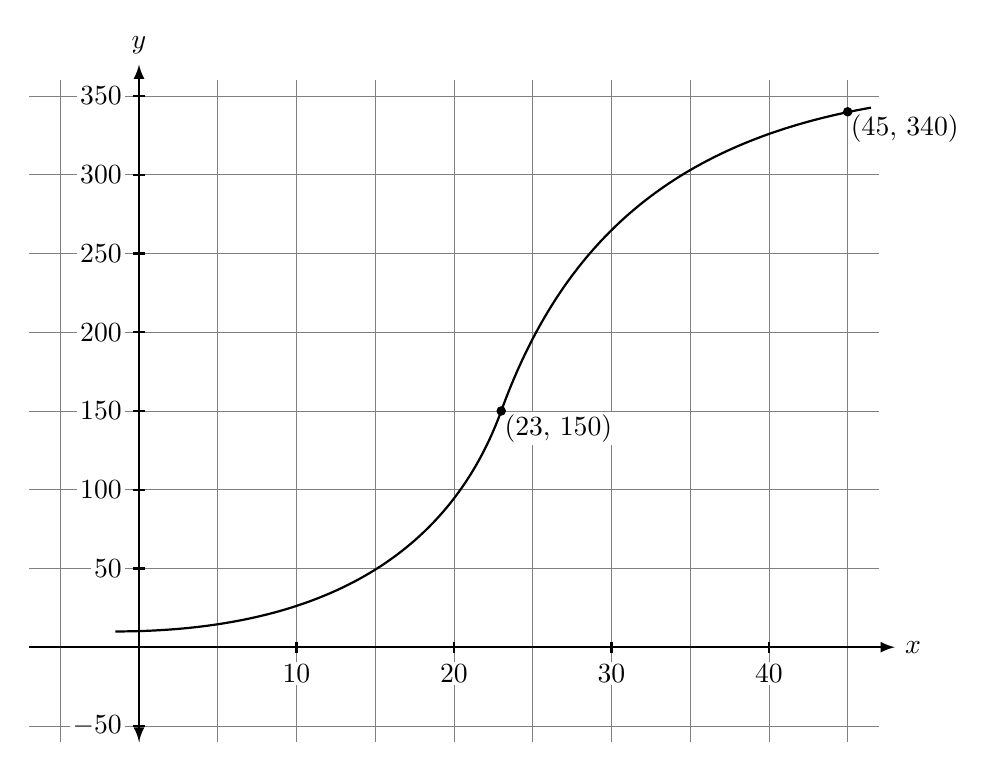
\begin{tikzpicture}[xscale=.20,yscale=.20]
    \draw[step=5,style=help lines,] (-7,-6) grid (47,36);
    \draw[-latex, thick] (-7,0)--(48,0) node[right]{$x$};
    \draw[latex-latex, thick] (0,-6)--(0,37) node[above]{$y$};
    
    \foreach \x/\xtext in {10,20,30,40} \draw[shift={(\x,0)},thick] (0pt,10pt) -- (0pt, -10pt) node[below=1mm,fill=white,inner sep=1pt]{$\xtext$};
    
    \foreach \y/\ytext in {5,10,15,20,25,30,35,-5} \draw[shift={(0,\y)},thick] (10pt,0pt) -- (-10pt, 0pt) node[left=1mm,fill=white,inner sep=1pt]{$\ytext0$};
  
    
    \node at (23,15)[anchor=north west,fill=white,inner sep=1pt]{$(23,\,150)$};
    \node at (45,34) [anchor=north west,fill=white,inner sep=1pt] {$(45,\,340)$};
    \node[circle,draw=black, fill=black, inner sep=0pt,minimum size=3pt] at (23,15) {};
    \node[circle,draw=black, fill=black, inner sep=0pt,minimum size=3pt] at (45,34) {};
    
    \draw[-,thick,shorten <=-.3cm] (0,1) to [out=0,in=250] (23,15);
    \draw[-,thick,shorten >=-.3cm] (23,15) to[out=70,in=-170] (45,34);
\end{tikzpicture}

A line through two points on a curve is called a \textbf{secant} to the curve. The slope of the secant line is the average rate of change.\\
\\
\\
\\
Did the number of flies increase by 8.6 each day?\\
\\
\\
\\
How fast was the fly population growing on day 23?

\newpage

The population growth on one particular day poses a problem: it would be the slope of the line at \textit{only one point}. We need \textit{two} points to use the slope formula as we know it. How do we circumvent this issue?\\
\\
\\
\textbf{Example:} Given $y=x^2$, what is the average rate of change on $[0,\,3]$?

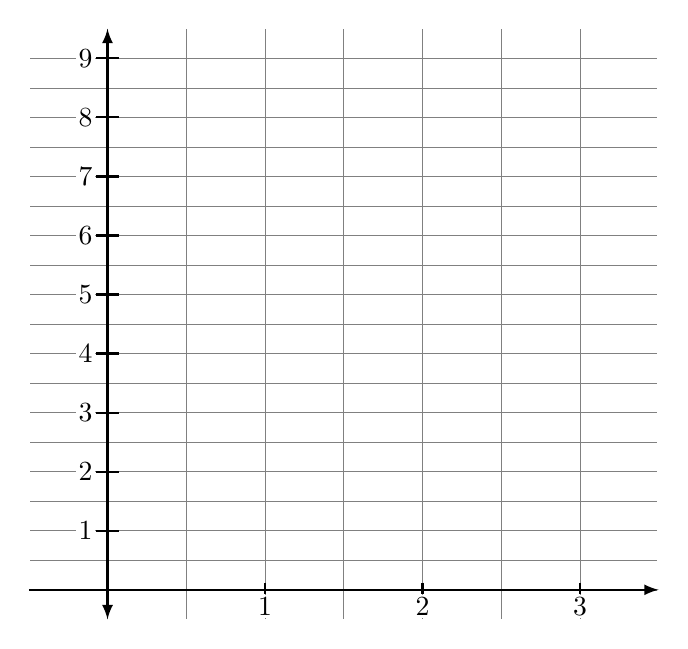
\begin{tikzpicture}[xscale=2,yscale=.75]
  \draw[step=.5,style=help lines] (-.49,-.49) grid (3.49,9.49);
  \draw[-latex, thick] (-.5,0)--(3.5,0);
  \draw[latex-latex, thick] (0,-.5)--(0,9.5);
  
  \foreach \x/\xtext in {1,2,3} \draw[shift={(\x,0)},thick] (0pt,3.5pt) -- (0pt, -2pt) node[below,fill=white,inner sep=1pt]{$\xtext$};
    
  \foreach \y/\ytext in {1,2,3,4,5,6,7,8,9} \draw[shift={(0,\y)},thick] (2pt,0pt) -- (-2pt, 0pt) node[left,fill=white,inner sep=1pt]{$\ytext$};
  
\end{tikzpicture}

What is the instantaneous rate of change at $x=1$?

\newpage


\begin{tcolorbox}[title= DEFINITION OF TANGENT LINE WITH SLOPE \textit{m},colframe=black,sharp corners,colback=white,colbacktitle=white,coltitle=black,boxrule=1pt]

    If $f$ is defined on an open interval containing $c$, and if the limit
    \[\lim_{\Delta x\to0}\frac{\Delta y}{\Delta x}=\lim_{\Delta x\to0}\frac{f(c+\Delta x)-f(c)}{\Delta x}=m\]
    exists, then the line passing through $(c,\,f(c))$ with slope $m$ is the \textbf{tangent line} to the graph of $f$ at the point $(c,\,f(c))$.
    
\end{tcolorbox}
\vspace{.15cm}
\noindent\textbf{Examples:}
\begin{questions}
    \question Write the equation of the tangent line to the curve $f(x)=3x^2+1$ at $x=-1$. 
    \vspace{\stretch{1}}
    
    \question Write a general formula for the slope of the tangent line to $f(x)=2x^2-x$ for any point $x=a$.
    \vspace{\stretch{1}}
    
    \question Write an equation for the line \textbf{normal} to the curve $f(x)=4-x^2$ at $x=1$.
    \vspace{\stretch{1}}
    
    \question Find the equations of all lines tangent to $y=9-x^2$ that pass through $(1,\,12)$.
    \vspace{\stretch{1.2}}
\end{questions}


\newpage
